\chapter{Planar Parameterization of Triangulated Surface Meshes}
\label{chap:surface_mesh_parameterization}
\ccChapterAuthor{Laurent Saboret, Pierre Alliez \and Bruno L\'evy}

\begin{ccPkgDescription}{Planar Parameterization of Triangulated Surface Meshes}
\ccPkgSummary{Parameterizing a surface amounts to finding a one-to-one mapping from
a suitable domain to the surface. In this package, we focus on
triangulated surfaces that are homeomorphic to a disk and on piecewise
linear mappings into a planar domain.  This \cgal\ package implements
some of the state-of-the-art surface mesh parameterization methods,
such as Least Squares Conformal Maps, Discrete Conformal Map, Discrete
Authalic Parameterization, Floater Mean Value Coordinates or Tutte
Barycentric Mapping.}

\ccPkgDependsOn{Solvers as \ccc{OpenNL} or \ccc{Taucs}.}
\ccPkgMaturity{Introduced in \cgal 3.2}

\end{ccPkgDescription}


\minitoc

This chapter describes \cgal's interpolation package which implements
natural neighbor coordinate functions as well as different
methods for scattered data interpolation most of which are based on
natural neighbor coordinates. The functions for the natural neighbor 
coordinates in Euclidian space are described in 
Section~\ref{sec:coordinates}, 
the functions concerning the coordinate and neighbor 
computation on surfaces are discussed in Section~\ref{sec:surface}. 
In Section~\ref{sec:interpolation}, we briefly describe the different interpolation functions.   

Scattered data interpolation solves the following problem: given
measures of a function on a set of discrete data points, the task is
to interpolate this function on an arbitrary query point.
More formally, let $\mathcal{P}=\{\mathbf{p_1},\ldots ,\mathbf{p_n}\}$ be a set of
$n$ point in $\mathbb{R}^2$ or $\mathbb{R}^3$ and $\Phi$ be a scalar
function defined inside the convex hull of $\mathcal{P}$. We assume that
the function values are known at the points of $\mathcal{P}$, i.e. to
each $\mathbf{p_i} \in \mathcal{P}$, we associate $z_i =
\Phi(\mathbf{p_i})$. Sometimes, the gradient of $\Phi$ is also known
at $\mathbf{p_i}$. It is denoted $\mathbf{g_i}= \nabla
\Phi(\mathbf{p_i})$. The interpolation is carried out for a point
$\mathbf{x}$ in the convex hull of $\mathcal{P}$.


\section{Basics}


\subsection{Default Surface Parameterization}

From the user point of view, the simplest entry point to this package
is the following function:

\ccFunction{Parameterizer_traits_3<ParameterizationMesh_3>::Error_code parameterize (ParameterizationMesh_3 & mesh);}
{
Compute a one-to-one mapping from a 3D triangle surface mesh to a 2D circle, using Floater Mean Value Coordinates algorithm. A one-to-one piecewise linear mapping is guaranteed. The result is a pair of (u,v) parameter coordinates for each vertex of the input mesh.\\
Preconditions: mesh must be a triangle mesh surface with one connected component.}

The function \ccc{CGAL::parameterize()} applies a default surface parameterization
method: Floater Mean Value Coordinates~\cite{cgal:f-mvc-03}, with an
arc-length circular border parameterization, and using OpenNL sparse
linear solver~\cite{cgal:l-nmdgp-05}. The \ccc{ParameterizationMesh_3} concept defines the input meshes handled by \ccc{CGAL::parameterize()}. See Section \ref{sec:Input-Mesh-for-parameterize}. The result is stored into the (u,v) fields of the mesh halfedges.

Note: \ccc{CGAL::Parameterizer_traits_3<ParameterizationMesh_3>} is the (pure virtual) superclass of all surface parameterizations and defines the error codes.


\subsection{Input Mesh for parameterize() \label{sec:Input-Mesh-for-parameterize}}

The input meshes handled \emph{directly} by \ccc{CGAL::parameterize()} must be models of \ccc{ParameterizationMesh_3}, triangulated, 2-manifold, oriented, and homeomorphic to discs (possibly with holes).

Note: \ccc{ParameterizationMesh_3} is a general concept to access a
polyhedral mesh. It is optimized for the \ccc{Surface_mesh_parameterization} package
only in the sense that it
defines the accessors to fields specific to the parameterization domain
(\ccc{index}, \ccc{u}, \ccc{v}, \ccc{is_parameterized}).
The extra constraints  needed by the surface parameterization methods (triangulated,
2-manifold, homeomorphic to a disc) are not part of the concept and
are checked at runtime.

This package provides a model of the \ccc{ParameterizationMesh_3} concept
to access \ccc{CGAL::Polyhedron_3<Traits>}: \\
\ccc{CGAL::Parameterization_polyhedron_adaptor_3<Polyhedron_3_>}

We will see later that \ccc{CGAL::parameterize()} can support \emph{indirectly}
meshes that are not topological disks.


\subsection{Default Parameterization Example}

\ccc{Simple_parameterization.C} applies the default parameterization to a
\ccc{CGAL::Polyhedron_3<Traits>} mesh (must be a topological disk).
Eventually, it extracts the result from halfedges and prints it.

\ccIncludeExampleCode{Surface_mesh_parameterization/Simple_parameterization.C}


\subsection{Enhanced parameterize() function}

This package provides a second \ccc{CGAL::parameterize()} entry point
where the user can specify a parameterization method:

\ccFunction{Parameterizer_traits_3<ParameterizationMesh_3>::Error_code parameterize (ParameterizationMesh_3 & mesh, ParameterizerTraits_3 parameterizer);}
{
Compute a one-to-one mapping from a 3D triangle surface 'mesh' to a simple 2D domain. The mapping is piecewise linear on the triangle mesh. The result is a pair (u,v) of parameter coordinates for each vertex of the input mesh.
One-to-one mapping may be guaranteed or not, depending on the chosen \ccc{ParametizerTraits_3} algorithm.\\
Preconditions: 'mesh' must be a triangle surface mesh with one connected component, and the mesh border must be mapped onto a convex polygon (for fixed border parameterizations).}


\subsection{Introduction to the Package Concepts}

\subsubsection{The ParameterizerTraits\_3 concept}

This \cgal\ package implements some of the state-of-the-art
surface parameterization methods, such as Least Squares Conformal Maps,
Discrete Conformal Map, Discrete Authalic
Parameterization, Floater Mean Value Coordinates or Tutte Barycentric
Mapping. These methods are provided as models of the
\ccc{ParameterizerTraits_3} concept. See Section \ref{sec:Surface-Parameterization-Methods}.

Each of these surface parameterization methods is templated by
the input mesh type, a border parameterization and a solver:

% Insert image parameterizer_class_diagram_simplified.png/eps
% with title "A parameterizer UML class diagram (simplified)" and scale = 1:1
\begin{center}
    \label{Surface_mesh_parameterization-fig-parameterizer_class_diagram_simplified}
    % Image
    \begin{ccTexOnly}
        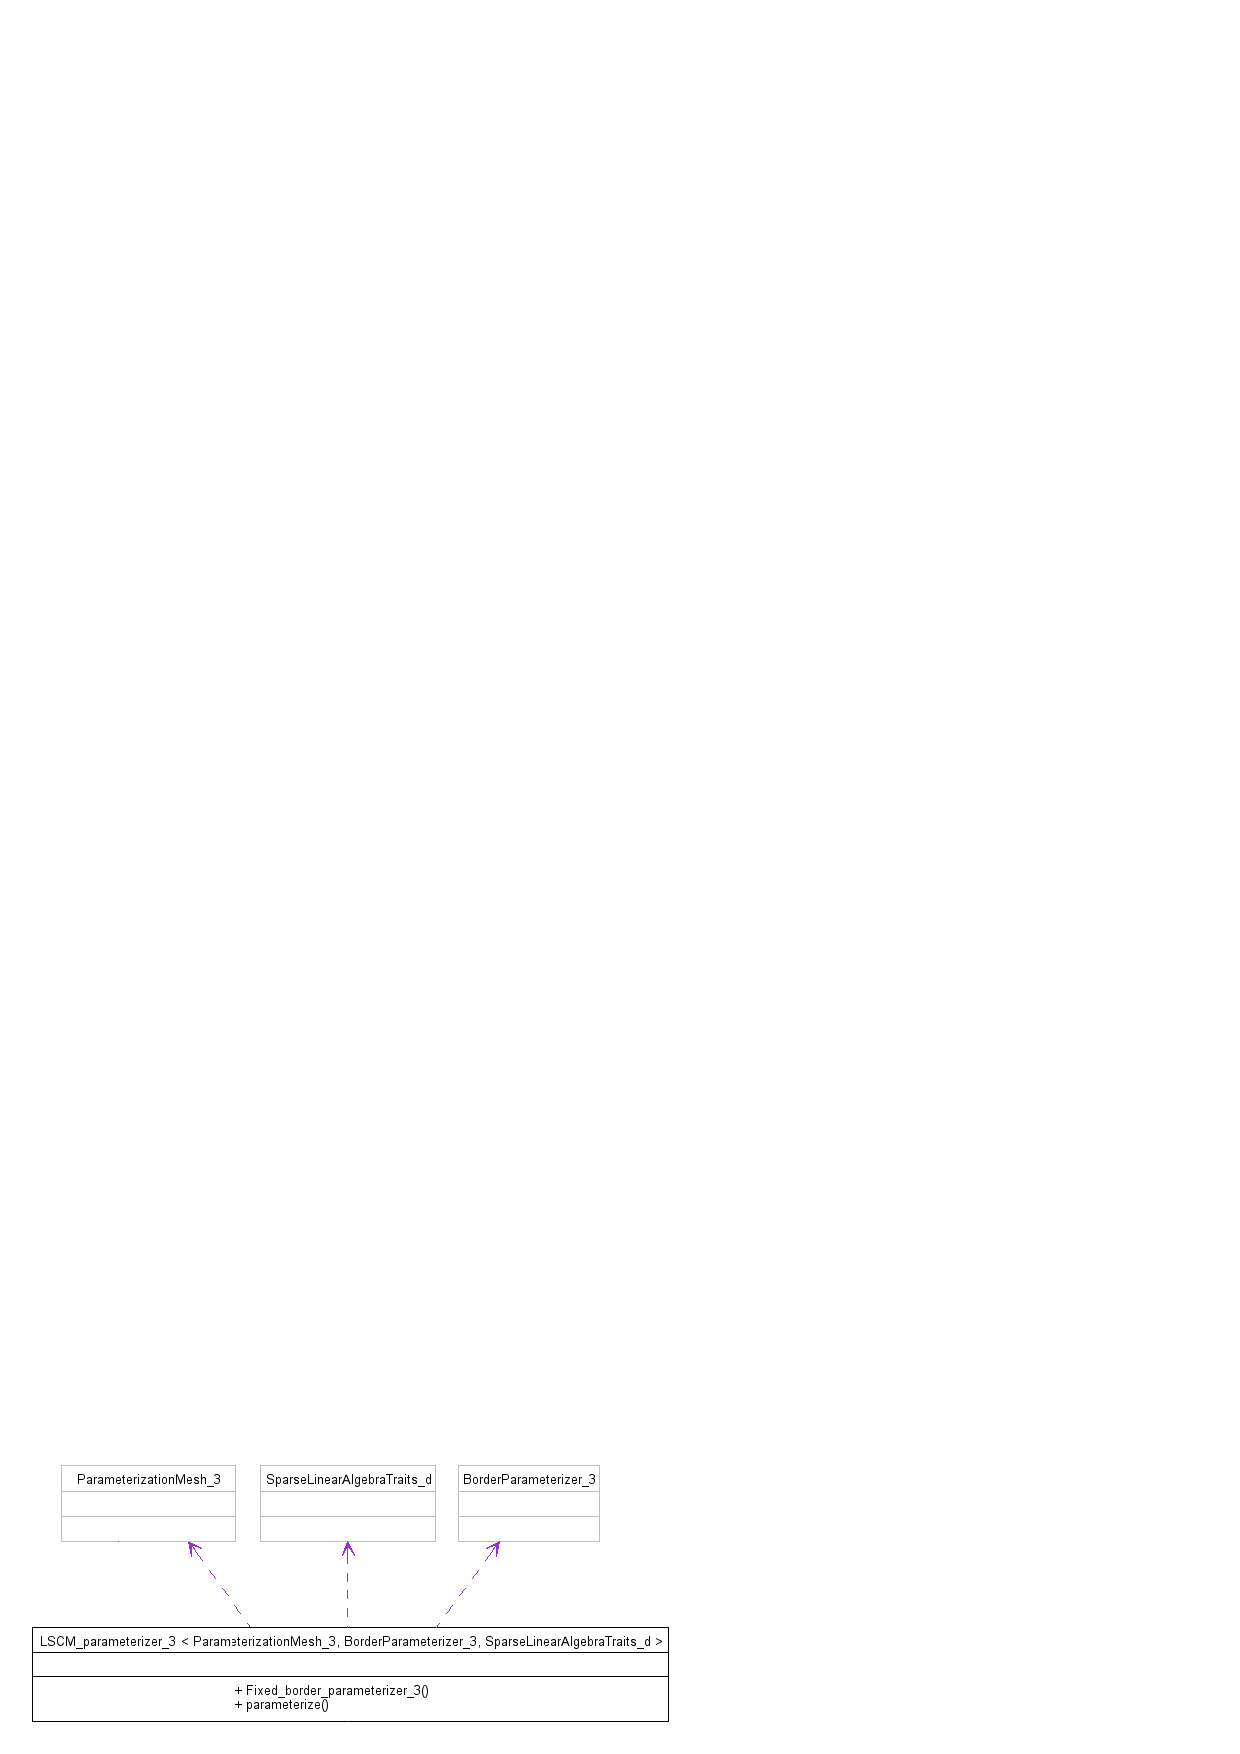
\includegraphics{Surface_mesh_parameterization/parameterizer_class_diagram_simplified} % omit .eps suffix
    \end{ccTexOnly}
    \begin{ccHtmlOnly}
        <img border=0 src="./parameterizer_class_diagram_simplified.png"><P>
    \end{ccHtmlOnly}
    % Title
    \begin{figure}[h]
        \caption{A parameterizer UML class diagram (simplified).}
    \end{figure}
\end{center}


\subsubsection{The BorderParameterizer\_3 concept}

Parameterization methods for
borders are used as traits classes modifying the behavior of
\ccc{ParameterizerTraits_3} models.
They are provided as models of the \ccc{BorderParameterizer_3} concept.
See Sections \ref{sec:Border-Parameterizations-for-Fixed-Methods}
and \ref{sec:Border-Parameterizations-for-Free-Methods}.


\subsubsection{The SparseLinearAlgebraTraits\_d concept}

This package solves sparse linear systems using solvers which are models
of \ccc{SparseLinearAlgebraTraits_d}. See Section \ref{sec:Sparse-Linear-Algebra}.


\subsubsection{The ParameterizationMesh\_3 and ParameterizationPatchableMesh\_3 Concepts}

As described in Section \ref{sec:Input-Mesh-for-parameterize}
the input meshes handled by \ccc{CGAL::parameterize()}
must be models of the \ccc{ParameterizationMesh_3} concept. The surface parameterization methods provided by this package only support
surfaces which are homeomorphic to disks, possibly with holes. Nevertheless meshed with arbitrary topology and number of connected components can be parameterized, provided that the user specifies a \emph{cut graph} (an oriented list of
vertices) which is the border of a topological disc. If no cut graph is
specified as input, the longest border of the input mesh is taken by default, the others being considered as holes.

For this purpose, the
\ccc{CGAL::Parameterization_mesh_patch_3<ParameterizationPatchableMesh_3>}
class is responsible for \emph{virtually} cutting
a patch into a \ccc{ParameterizationPatchableMesh_3} mesh.
The resulting patch is a topological
disk (if the input cutting path is correct)
and provides a \ccc{ParameterizationMesh_3} interface. It can be used as
parameter for the function \ccc{CGAL::parameterize()}.

\ccc{ParameterizationPatchableMesh_3} inherits from \ccc{ParameterizationMesh_3},
thus is a concept for a 3D surface mesh.
\ccc{ParameterizationPatchableMesh_3} adds the ability to support patches and
virtual seams. \emph{Patches} are a subset of a 3D mesh.
\emph{Virtual seams} behave as if the surface was cut along a cut graph. More information is provided in Section \ref{sec:Cutting-a-Mesh}.

\section{Surface Parameterization Methods}


This package provides a second \ccc{parameterize()} entry point
where the user can specify a parameterization method:

\ccFunction{Parameterizer_traits_3<ParameterizationMesh_3>::Error_code parameterize (ParameterizationMesh_3 * mesh, ParameterizerTraits_3 parameterizer);}
{ Compute a ont-to-one mapping from a 3D triangle surface 'mesh' to a
simple 2D domain. The mapping is piecewise linear on the triangle
mesh. The result is a pair (u,v) of parameter coordinates for each
vertex of the input mesh.  One-to-one mapping may be guaranteed or
not, depending on the chosen ParametizerTraits\_3 algorithm.
Preconditions:\begin{itemize} 
\item 'mesh' must be a surface with one connected component.\item
'mesh' must be a triangle mesh.\item the mesh boundary must be mapped
onto a convex polygon (for fixed border
parameterizations).\end{itemize} }


This \cgal\ package implements some of the state-of-the-art surface
parameterization methods which can be used as
\ccc{ParameterizerTraits_3} parameter. This package also provides common parameterization methods for
boundaries which are used as traits classes modifying the behavior of
the \ccc{ParameterizerTraits_3} methods.


\subsection{Fixed Border Surface Parameterizations}

% pierre: I would replace border by boundary everywhere

Fixed Border Surface Parameterizations need a set of constraints: two
u,v coordinates for each vertex along the boundary. Some helper
functions to achieve this goal are described in Section xxx.

% pierre: add ref

\subsubsection{Tutte Barycentric Mapping}

\ccc{CGAL::Barycentric_mapping_parameterizer_3}  \\

The Barycentric Mapping parameterization method has been introduced by
Tutte~\cite{cgal:fh-survey-05}. In parameter space, each vertex is
placed at the barycenter of its neighbors to achieve the so-called
convex combination condition. This amounts to solve one
sparse linear solver for each set of parameter coordinates, with a
\#vertices x \#vertices sparse and symmetric positive definite matrix. 
A coefficient $(i,j)$ of the matrix is set to 1 for an edge linking
the vertex $v_i$ to the vertex $v_j$, to minus the degree of the
vertex $v_i$ for a diagonal element, and to zero for any other matrix
entry. Although Tutte Barycentric Mapping method is fast and
guaranteed to be bijective, it does not minimize angle nor area
distortion.

% pierre: reference Tutte's paper, not survey

% Include uniform.png/eps figure with title =
% "Tutte Barycentric Mapping (the red line emphasizes the cutting path)"
\begin{figure}[bht]
    \begin{center}
        % Image
        \begin{ccTexOnly}
            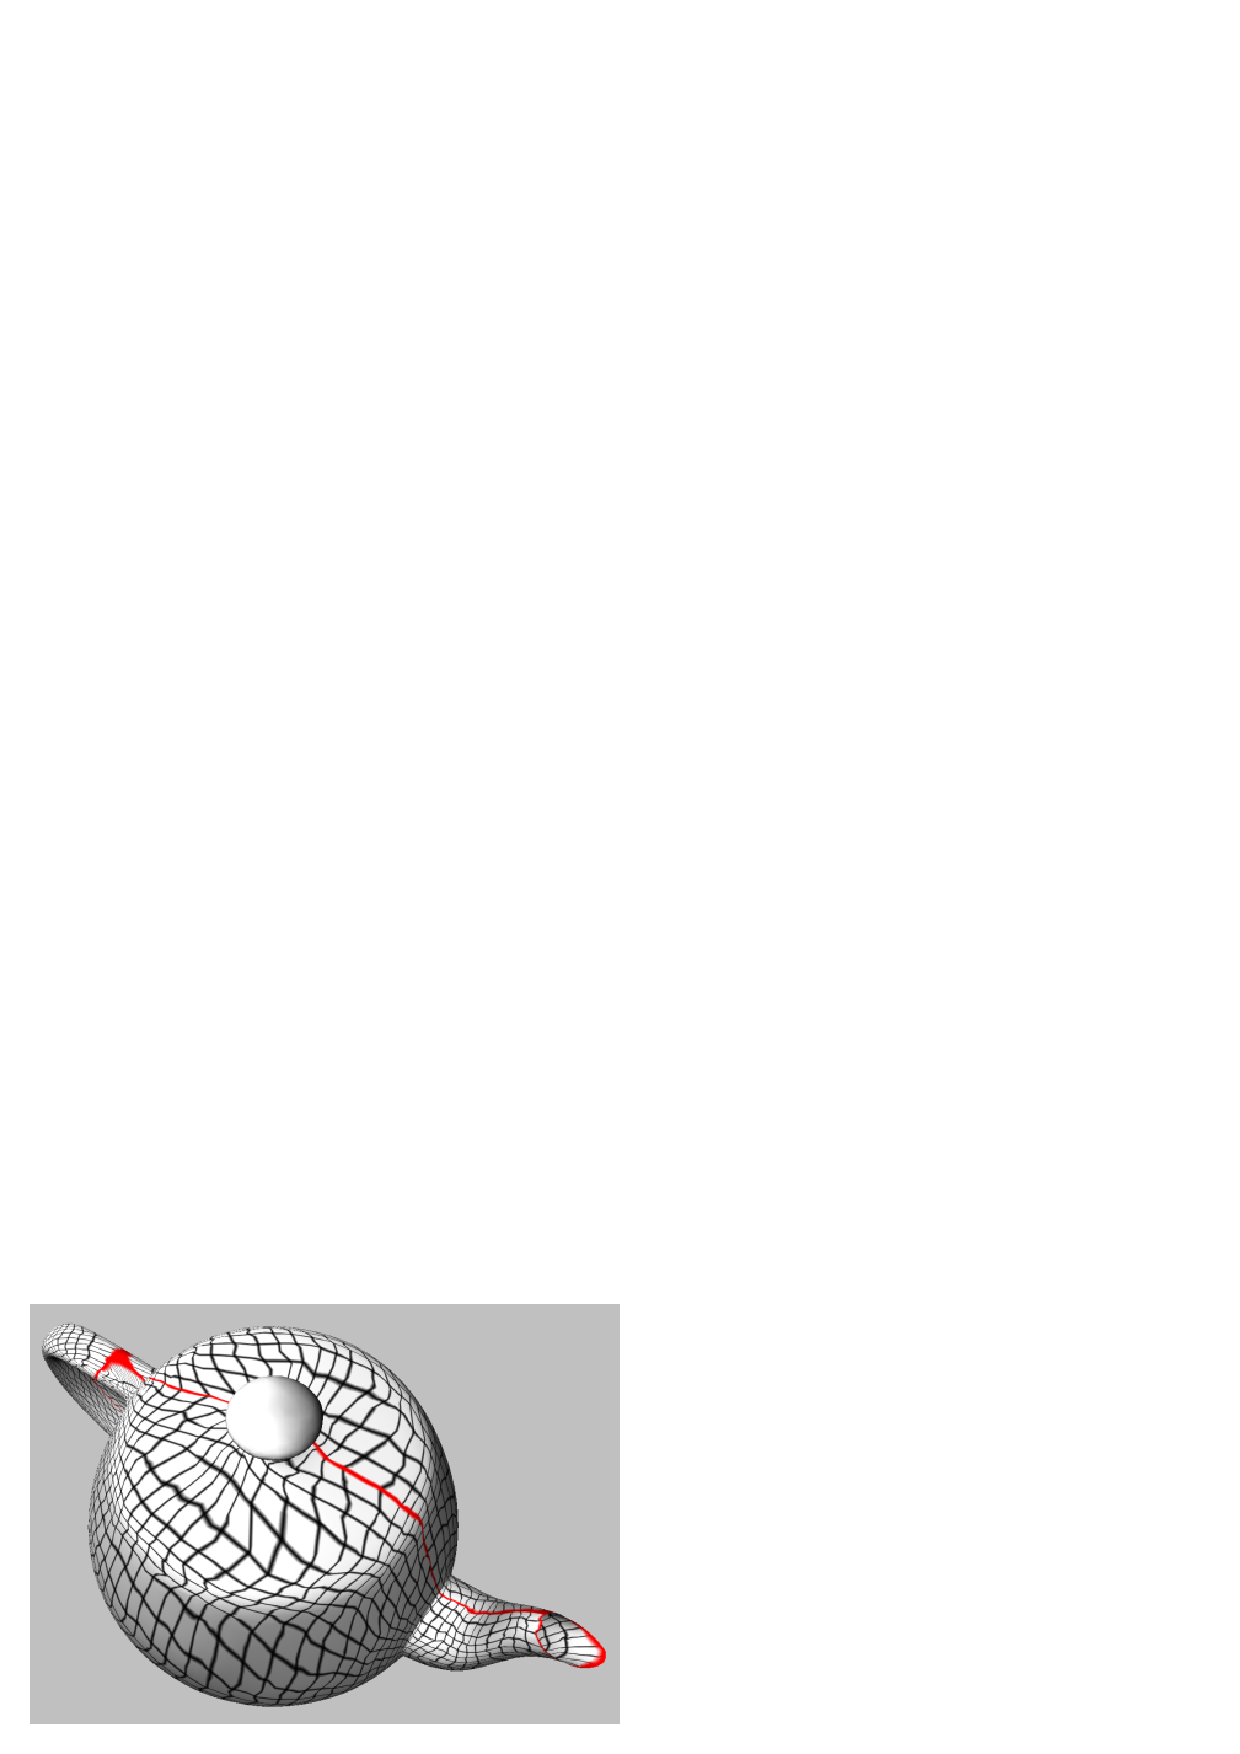
\includegraphics{Parameterization/uniform} % omit suffix to support PS and PDF
        \end{ccTexOnly}
        \begin{ccHtmlOnly}
            <img border=0 src="./uniform.png" align=center>
        \end{ccHtmlOnly}
        \label{parameterization-fig-uniform}

        % Title
        \caption{Tutte Barycentric Mapping (the red line emphasizes the cutting path)}
    \end{center}
\end{figure}


\subsubsection{Discrete Conformal Map}

\ccc{CGAL::Discrete_conformal_map_parameterizer_3}  \\

Discrete Conformal Map parameterization has been introduced by Eck et
al. to he graphics community~\cite{cgal:fh-survey-05}. It attempts to
lower angle deformation by minimizing a discrete version of the
Dirichlet energy as derived by Pinkall and
Polthier~\cite{cgal:fh-survey-05}.

% pierre: fix references

A one-to-one mapping is guaranteed only when two conditions are
fulfilled: the barycentric mapping condition (each vertex in parameter
space is a convex combination if its neighbouring vertices) and the
boundary is convex.

% pierre: add cot figure, and detail what it means to have all weights
% positive, otherwise it is confusing.

This method solves two \#vertices x \#vertices sparse linear
systems. The matrix (the same for both systems) is symmetric definite
positive, thus can be efficiently solved using dedicated linear
solvers (x s for the example shown).

% Include conformal.png/eps figure with title = "Discrete Conformal Map"
\begin{figure}[bht]
    \begin{center}
        % Image
        \begin{ccTexOnly}
            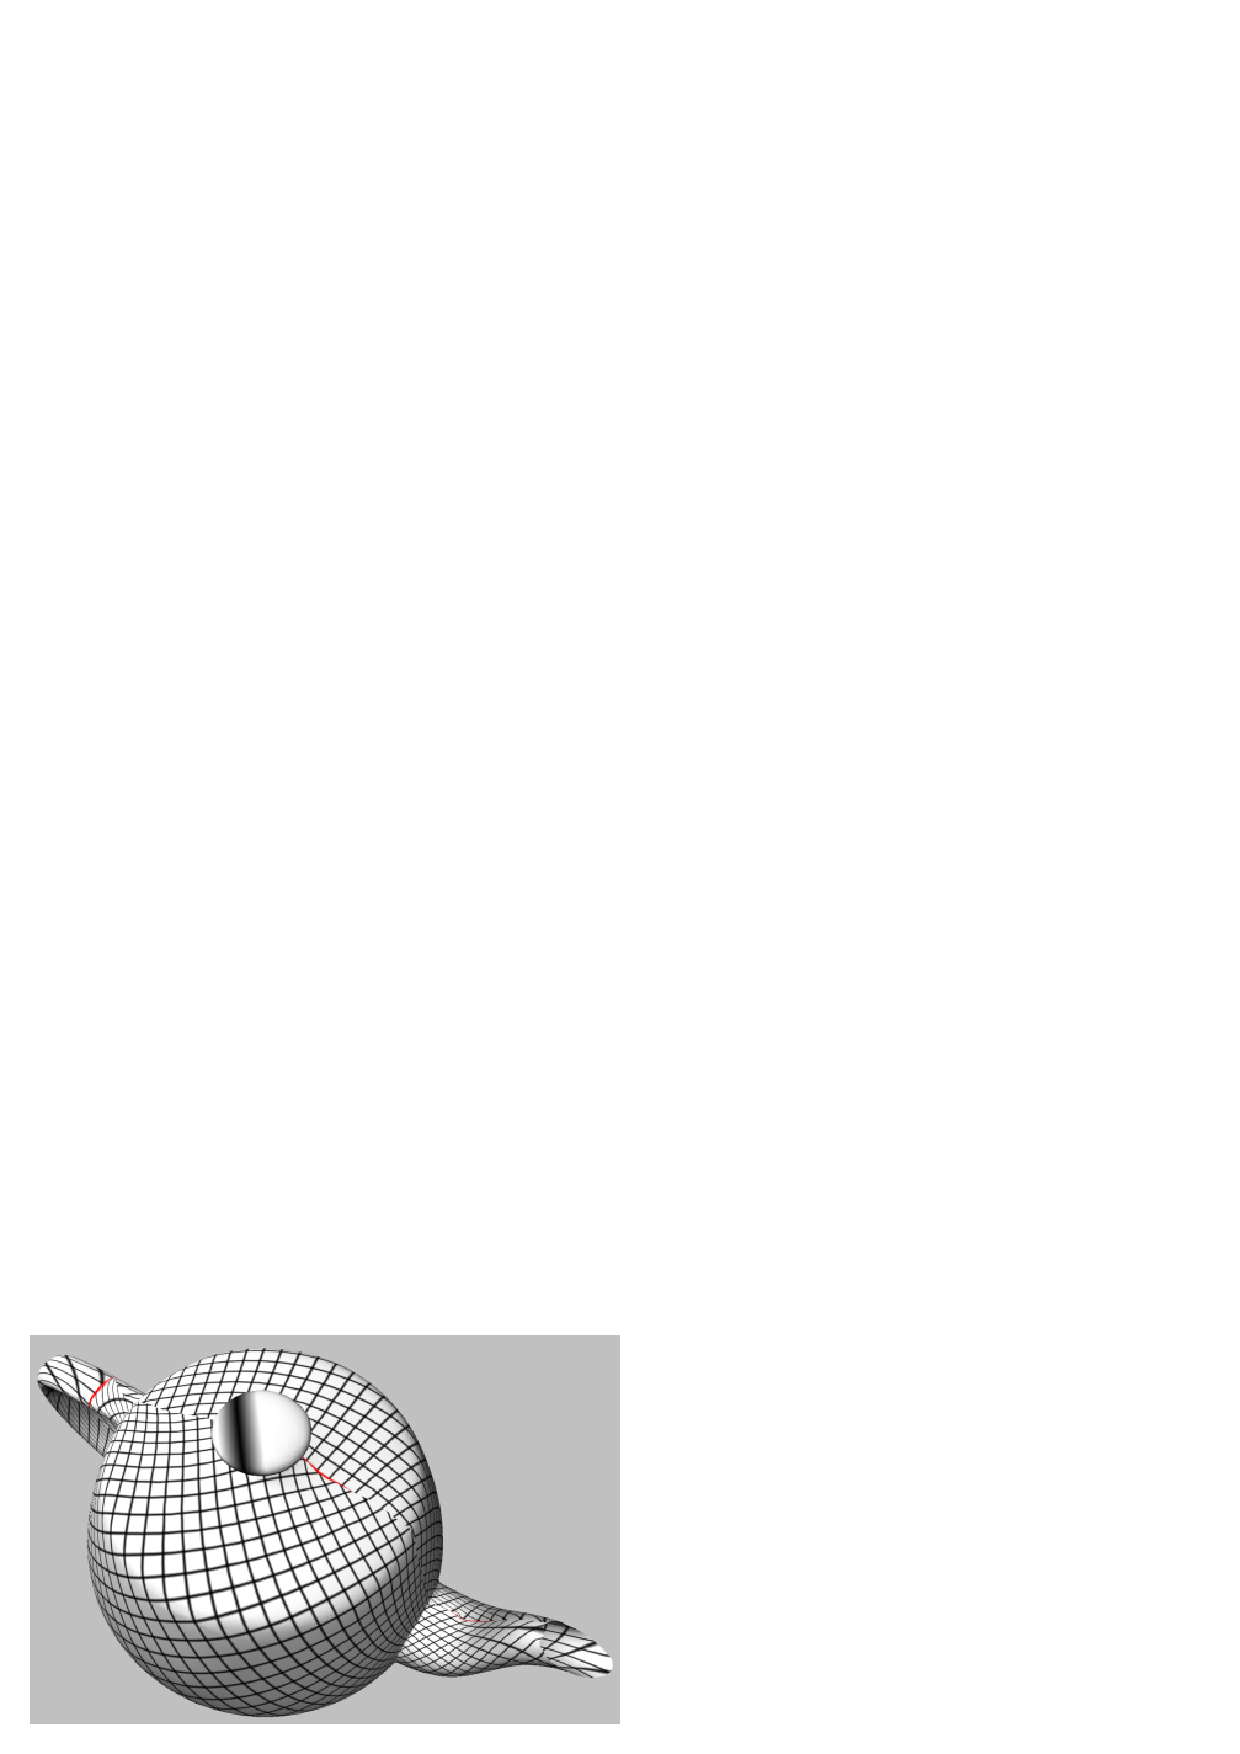
\includegraphics{Parameterization/conformal} % omit suffix to support PS and PDF
        \end{ccTexOnly}
        \begin{ccHtmlOnly}
            <img border=0 src="./conformal.png" align=center>
        \end{ccHtmlOnly}
        \label{parameterization-fig-conformal}

        % Title
        \caption{Discrete Conformal Map}
    \end{center}
\end{figure}


\subsubsection{Floater Mean Value Coordinates}

\ccc{CGAL::Mean_value_coordinates_parameterizer_3}  \\

The Mean Value Coordinates parameterization method has been introduced
by Floater~\cite{cgal:f-mvc-03}. Each vertex in parameter space is
optimized so as to be a convex combination of its neighbouring
vertices. The barycentric coordinates are this time unconditionnaly
positive, by deriving an application of the mean theorem for harmonic
functions. It is in essence an approximation of the Discrete Conformal
Maps, with a one-to-one mapping always guaranteed. This method solves
two \#vertices x \#vertices sparse linear systems. The matrix (the
same for both systems) is asymmetric.

% Include floater.png/eps figure with title = "Floater Mean Value Coordinates"
\begin{figure}[bht]
    \begin{center}
        % Image
        \begin{ccTexOnly}
            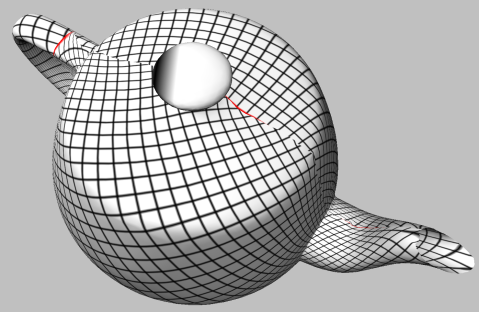
\includegraphics{Parameterization/floater} % omit suffix to support PS and PDF
        \end{ccTexOnly}
        \begin{ccHtmlOnly}
            <img border=0 src="./floater.png" align=center>
        \end{ccHtmlOnly}
        \label{parameterization-fig-floater}

        % Title
        \caption{Floater Mean Value Coordinates}
    \end{center}
\end{figure}


\subsubsection{Discrete Authalic parameterization}

\ccc{CGAL::Discrete_authalic_parameterizer_3}  \\

The Discrete Authalic parameterization method has been introduced by
Desbrun, Meyer and Alliez~\cite{cgal:dma-ipsm-02}.  It corresponds to
a weak formulation of an area-preserving method, and in essence
locally minimizes the area distortion. A one-to-one mapping is
guaranteed only if the convex combination condition is fulfilled and
the boundary is convex.  This method solves two
\#vertices x \#vertices sparse linear systems. The matrix (the same
for both systems) is asymmetric.

% Include authalic.png/eps figure with title = "Discrete Authalic Parameterization"
\begin{figure}[bht]
    \begin{center}
        % Image
        \begin{ccTexOnly}
            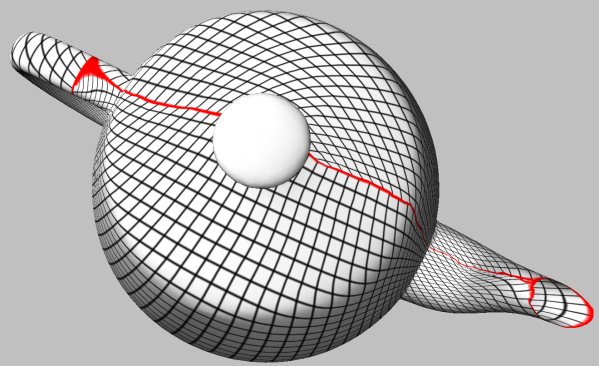
\includegraphics{Parameterization/authalic} % omit suffix to support PS and PDF
        \end{ccTexOnly}
        \begin{ccHtmlOnly}
            <img border=0 src="./authalic.png" align=center>
        \end{ccHtmlOnly}
        \label{parameterization-fig-authalic}

        % Title
        \caption{Discrete Authalic Parameterization}
    \end{center}
\end{figure}


\subsubsection{Associated Border Parameterization}

Border Parameterizations for Fixed Border Surface Parameterizations
are a family of methods to define a set of constraints, namely two
$u,v$ coordinates for each vertex along the boundary.

\begin{itemize}

\item The user can select a border parameterization among
two commonly used methods: uniform or arc-length parameterization, the
arc-length parameterization being used by default.

\item One convex shape specified by:

    \begin{itemize}

    \item one shape among two standard ones: a circle or a square.
    The circular boundary parameterization is used by default as it
    corresponds to the simplest convex shape. The square border
    parameterization is commonly used for texture mapping.

    \item a convex polygon.

    (not yet implemented)

    \end{itemize}

\end{itemize}

\ccc{CGAL::Circular_border_arc_length_parameterizer_3}  \\
\ccc{CGAL::Circular_border_uniform_parameterizer_3}  \\
\ccc{CGAL::Square_border_arc_length_parameterizer_3}  \\
\ccc{CGAL::Square_border_uniform_parameterizer_3}  \\


\subsection{Free Border Surface Parameterizations}

\subsubsection{Least Squares Conformal Maps}

\ccc{CGAL::LSCM_parameterizer_3}  \\

The Least Squares Conformal Maps (LSCM) parameterization method has
been introduced by L\'evy et al.~\cite{cgal:lprm-lscm-02}. It
corresponds to a conformal method with a free boundary (at least two
vertices have to be constrained to obtain a unique solution), which
allows further lowering of the angle distortion. A one-to-one mapping
is not guaranteed by this method. It solves a (2 $\times$
\#triangles) $\times$ \#vertices sparse linear system in the least squares sense.

% Include LSCM.png/eps figure with title = "Least Squares Conformal Maps"
\begin{figure}[bht]
    \begin{center}
        % Image
        \begin{ccTexOnly}
            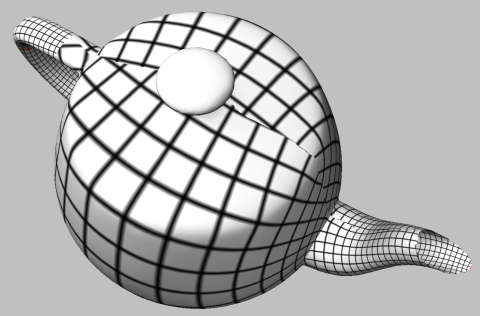
\includegraphics{Parameterization/LSCM} % omit suffix to support PS and PDF
        \end{ccTexOnly}
        \begin{ccHtmlOnly}
            <img border=0 src="./LSCM.png" align=center>
        \end{ccHtmlOnly}
        \label{parameterization-fig-LSCM}

        % Title
        \caption{Least Squares Conformal Maps}
    \end{center}
\end{figure}


\subsubsection{Natural Conformal Map}

(not yet implemented)

The Natural Conformal Map parameterization method has been introduced
by Desbrun et al.~\cite{cgal:dma-ipsm-02}. It extends the Discrete
Conformal Map method by optimizing the boundary vertices in addition
to the interior vertices, as already achived by the LSCM method
described above. At least two vertices have to be constrained to
obtain a unique solution. This method solves a (2 $\times$ \#vertices) $\times$
\#vertices sparse linear system.  The matrix is symmetric definite
positive, thus can be efficiently solved.

% pierre: double check that it is indeed symmetric!


\subsubsection{Associated Border Parameterization}

\ccc{CGAL::Two_vertices_parameterizer_3}  \\

The associated Border Parameterization method defines only two constraints
(the pinned vertices). They have to be on the specified boundary.


\subsection{Discrete Authalic Parameterization Example}

The following C++ code computes a Discrete Authalic parameterization
to a \ccc{Polyhedron_3} mesh:

\begin{ccExampleCode}

// CGAL kernel
typedef CGAL::Cartesian<double>                         Kernel;

// Mesh true type and parameterization adaptors
typedef CGAL::Polyhedron_3<Kernel>                      Polyhedron;
typedef CGAL::Parameterization_polyhedron_adaptor_3<Polyhedron>
                                                        Parameterization_polyhedron_adaptor;

// Discrete Authalic Parameterization
typedef CGAL::Discrete_authalic_parameterizer_3<Parameterization_polyhedron_adaptor>
                                                        Parameterizer;

int main(int argc,char * argv[])
{
    Polyhedron mesh;
    ...

    // The parameterization package needs an adaptor to handle Polyhedron_3 meshes
    // The mesh must be a topological disk
    Parameterization_polyhedron_adaptor mesh_adaptor(&mesh);

    // Discrete Authalic Parameterization
    Parameterizer::Error_code err = CGAL::parameterize(&mesh_adaptor, Parameterizer());
    ...
}

\end{ccExampleCode}

The complete example is available in
\ccc{Authalic_parameterization.C}.


\subsection{Square Border Arc Length Parameterization Example}

The following C++ code computes a Floater Mean Value Coordinates
parameterization with a Square Border Arc Length parameterization:

\begin{ccExampleCode}

// CGAL kernel
typedef CGAL::Cartesian<double>                         Kernel;

// Mesh true type and parameterization adaptors
typedef CGAL::Polyhedron_3<Kernel>                      Polyhedron;
typedef CGAL::Parameterization_polyhedron_adaptor_3<Polyhedron>
                                                        Parameterization_polyhedron_adaptor;

// Square border parameterizer
typedef CGAL::Square_border_arc_length_parameterizer_3<Parameterization_polyhedron_adaptor>
                                                        Border_parameterizer;

// Floater Mean Value Coordinates parameterizer with square border
typedef CGAL::Mean_value_coordinates_parameterizer_3<Parameterization_polyhedron_adaptor,
                                                     Border_parameterizer>
                                                        Parameterizer;

int main(int argc,char * argv[])
{
    Polyhedron mesh;
    ...

    // The parameterization package needs an adaptor to handle Polyhedron_3 meshes
    // The mesh must be a topological disk
    Parameterization_polyhedron_adaptor mesh_adaptor(&mesh);

    // Floater Mean Value Coordinates parameterization
    // with a Square Border Arc Length Parameterization
    Parameterizer::Error_code err = CGAL::parameterize(&mesh_adaptor, Parameterizer());
    ...
}

\end{ccExampleCode}

See the complete example \ccc{Square_border_parameterization.C}.

\section{Sparse Linear Algebra}

\subsection{Solvers List and Concept}

We provide an interface to several state-of-the-art
sparse linear solvers, as models of the SparseLinearAlgebraTraits\_d concept:

\begin{itemize}

\item OpenNL (Bruno L{\'e}vy) is shipped with \cgal. This is the default solver.

OpenNL::DefaultLinearSolverTraits  \\
OpenNL::SymmetricLinearSolverTraits  \\

\item TAUCS is a reference direct solver for sparse symmetric matrices.

\ccRefIdfierPage{CGAL::Taucs_solver_traits}  \\
\ccRefIdfierPage{CGAL::Taucs_symmetric_solver_traits}  \\

\item SuperLU is a reference direct solver for sparse unsymmetric matrices.

(traits class not yet implemented)

\end{itemize}


\subsection{TAUCS Solver Example}

The code above uses the default sparse linear solver: OpenNL.

The code below applies the default parameterization method
(Floater's mean value coordinates with a circular border),
but specifically instantiates TAUCS solver:

\begin{ccExampleCode}

// CGAL kernel
typedef CGAL::Cartesian<double>                         Kernel;

// Mesh true type and parameterization adaptors
typedef CGAL::Polyhedron_3<Kernel>                      Polyhedron;
typedef CGAL::Mesh_adaptor_polyhedron_3<Polyhedron>     Mesh_adaptor_polyhedron;

// Circular border parametizer (the default)
typedef CGAL::Circular_border_arc_length_parametizer_3<Mesh_adaptor_polyhedron>
                                                        Border_parametizer;
// TAUCS solver
typedef CGAL::Taucs_solver_traits<double>               Solver;

// Floater's mean value coordinates parametizer (circular border)
// with TAUCS solver
typedef CGAL::Mean_value_coordinates_parametizer_3<Mesh_adaptor_polyhedron,
                                                   Border_parametizer,
                                                   Solver>
                                                        Parametizer;

int main(int argc,char * argv[])
{
    Polyhedron mesh;
    ...

    // The parameterization package needs an adaptor to handle Polyhedron_3 meshes
    Mesh_adaptor_polyhedron mesh_adaptor(&mesh);

    // Floater's mean value coordinates parametizer (circular border)
    // with TAUCS solver
    Parametizer::Error_code err = CGAL::parameterize(&mesh_adaptor, Parametizer());
    ...
}

\end{ccExampleCode}

See the complete code in Polyhedron\_parameterization4.C example.


\section{Cutting a Mesh}

\subsection{Computing a Cut}

All surface parameterization methods proposed in this package only
deal with topological discs.  The input mesh can be of any genus and
have any number of connected components, but if it is not a topological
disc, it has to come with a description of a boundary (an oriented list of
vertices) which is the border of a topological disc.  If no boundary  is
given as input, we assume that the surface border is the longest border already
in the input mesh (the other borders will be considered as holes).

% pierre: big contradiction here - it can be something else than a
% disk then!

This package does not provide any algorithm to transform a closed mesh
of arbitrary genus into a topological disk, the user being responsible
for computing such a cut. Nevertheless we provide in
\ccc{polyhedron_ex_parameterization.C} a simple cutting algorithm for
the sake of completeness.


\subsection{Applying a Cut}

Parameterization methods in this package only support triangulated
surfaces that are homeomorphic to a disk (models of
\ccc{ParameterizationMesh_3}). This software design simplifies the
implementation of all new parameterization methods based on linear
solvers.

\ccc{Parameterization_mesh_patch_3} class is responsible for virtually
{\em cutting} a patch to a \ccc{ParameterizationPatchableMesh_3} mesh,
to make it similar ffromt he interface point of view to a topological
disk with a \ccc{ParameterizationMesh_3} interface.

\ccc{ParameterizationPatchableMesh_3} inherits from concept \ccc{ParameterizationMesh_3}, thus is a concept for a 3D surface mesh.
\ccc{ParameterizationPatchableMesh_3} adds the ability to support patches and virtual seams. Patches are a subset of a 3D mesh. Virtual seams are the ability to behave exactly as if the surface was {\em cut} following a certain path.

The \ccc{ParameterizationMesh_3} interfaces with both the 2D
Triangulation Data Structure enriched with 3D points (not yet
implemented) and the Polyhedron are also models of
\ccc{ParameterizationPatchableMesh_3}:

\ccc{CGAL::Parameterization_polyhedron_adaptor_3}  \\


\subsection{Cutting a Mesh Example}

The code below virtually {\em cuts} a \ccc{Polyhedron_3} mesh to make
it a topological disk, then applies the default parameterization:

\begin{ccExampleCode}

// CGAL kernel
typedef CGAL::Cartesian<double>                             Kernel;

// Mesh true type and parameterization adaptors
typedef CGAL::Polyhedron_3<Kernel>                          Polyhedron;
typedef CGAL::Parameterization_polyhedron_adaptor_3<Polyhedron>
                                                            Parameterization_polyhedron_adaptor;
typedef CGAL::Parameterization_mesh_patch_3<Parameterization_polyhedron_adaptor>
                                                            Mesh_patch_polyhedron;

// Parameterizers base class for this kind of mesh
typedef CGAL::Parameterizer_traits_3<Mesh_patch_polyhedron> Parameterizer;

// Type describing a border or seam as a vertex list
typedef std::list<Parameterization_polyhedron_adaptor::Vertex_handle>
                                                            Seam;

// If the mesh is a topological disk, extract its longest border,
// else compute a very simple cut to make it homeomorphic to a disk.
// Return the border/seam (empty on error)
static Seam cut_mesh(Parameterization_polyhedron_adaptor* mesh_adaptor)
{
    // To be implemented by package user
    ...
}

int main(int argc,char * argv[])
{
    Polyhedron mesh;
    ...

    // The parameterization package needs an adaptor to handle Polyhedron_3 meshes
    Parameterization_polyhedron_adaptor mesh_adaptor(&mesh);

    // The parameterization methods support only meshes that
    // are topological disks => we need to compute a "cutting" of the mesh
    // that makes it it homeomorphic to a disk
    Seam seam = cut_mesh(&mesh_adaptor);

    // Create adaptor that virtually "cuts" the mesh following the 'seam' path
    Mesh_patch_polyhedron   mesh_patch(&mesh_adaptor,
                                       seam.begin(),
                                       seam.end());

    // Floater Mean Value Coordinates parameterization
    Parameterizer::Error_code err = CGAL::parameterize(&mesh_patch);
    ...
}

\end{ccExampleCode}

See the complete example in \ccc{Mesh_cutting_parameterization.C}
example.



\section{Output}

The surface reconstructed by \ccc{make_surface_mesh()} is required to be a model of the concept \ccc{SurfaceMeshComplex_2InTriangulation_3}, a data structure devised to represent a two dimensional complex embedded into a three dimensional triangulation.

\ccc{SurfaceMeshComplex_2InTriangulation_3} defines the methods to traverse the reconstructed surface, and e.g. convert it to a triangle soup.

Other \cgal\ components provide functions to write the reconstructed surface mesh to the Object File Format (OFF)~\cite{cgal:p-gmgv16-96} and to convert it to a polyhedron (when it is manifold): \\
\ccc{CGAL::output_surface_facets_to_off}  \\
\ccc{CGAL::output_surface_facets_to_polyhedron}  \\

See \ccc{poisson_reconstruction_example.cpp} example above.

\section{Complexity and Guarantees}


\subsection{Parameterization Methods and Guarantees}

\begin{itemize}

\item Fixed boundaries

    \begin{itemize}

    \item One-to-one mapping

        Tutte's theorem guarantees a one-to-one mapping provided that the weights are positive
        and the border convex.
        It is the case for Tutte Barycentric Mapping and Floater Mean Value Coordinates.
        It is not always the case for Discrete Conformal Map (cotangents) and
        Discrete Authalic Parameterization.

    \item Non-singularity of the matrix

        Geshorgin's theorem guarantees the convergence of the solver if the matrix is diagonal dominant.
        This is the case with positive weights (Tutte Barycentric Mapping and Floater Mean Value
        Coordinates).

    \end{itemize}

\item Free boundaries

    \begin{itemize}

    \item One-to-one mapping

        No guarantee can be given for LSCM (both global overlaps and triangle flips can
        occur).

    \item Non-singularity of the matrix

        Proven for LSCM: the matrix of the system is the Gramm matrix of a matrix of maximal rank,
        and is therefore non-singular (Gramm theorem).

    \end{itemize}

\end{itemize}


\subsection{Precision}

Only a few algorithms of this package construct the sparse linear system(s)
using trigonometric functions, incompatible with an exact arithmetic:

\begin{itemize}

\item Floater Mean Value Coordinates

\item Circular border parameterization

\end{itemize}

On the other hand, linear solvers commonly use double precision floating point
numbers. \\
OpenNL's BICGSTAB solver (accessible though the
\ccc{OpenNL::DefaultLinearSolverTraits<COEFFTYPE, MATRIX, VECTOR, SOLVER>} interface)
is the only solver supported by this package that
computes exact results (when used with an exact arithmetic).

Therefore, this package is intended to be used with a \cgal\
cartesian kernel with doubles.


\subsubsection{OpenNL's BICGSTAB Solver with an Exact Arithmetic}

The BICGSTAB conjugate gradient is in fact a direct solver.
In a nutshell, it computes a vector basis
orthogonal with respect to the matrix, and the coordinates of the solution in this vector basis.
Each iteration computes one component of the basis and one coordinate, therefore the algorithm
converges to the solution in $n$ iterations, where $n$ is the dimension of the matrix.
In fact, it can be even less than $n$, it converges in $k$ iteration, where $k$ is the number
of distinct eigenvalues of the matrix. \\
\emph{Note:} for a perfectly conditioned matrix, it converges in one iteration!


\subsubsection{Solvers with a Floating Point Arithmetic}

\emph{OpenNL's BICGSTAB example:}

When inexact numerical types are used (e.g. doubles), accumulated errors slow down convergence
(in practice, it requires approximately $5k$ iterations to converge).
The required number of iterations depends on the eigenvalues of the matrix, and these eigenvalues depend
on the shape of the triangles. The optimum is when the triangles are equilateral (then the solver converges
in less than 10 iterations). The worst case is obtained when the mesh has a large number of skinny triangles (near-singular Jacobian matrix of the triangle). In this case, the spectrum of the matrix
is wide (many different eigenvalues), and the solver requires nearly $5n$ iterations to converge.


\subsection{Algorithmic Complexity}

In this package, we focus on piecewise linear mappings onto a planar
domain. All surface parameterization methods are based on solving one (or two)
sparse linear system(s).
The algorithmic complexity is dominated by the resolution of the sparse linear system(s).

\emph{OpenNL's BICGSTAB example:}

At each iteration, the operation of highest complexity is the sparse-matrix x vector product.
The sparse matrix has a fixed number of non-zero coefficients per row,
therefore the sparse-matrix x vector product has $O(n)$ complexity.
Since convergence is reached after $k$ iterations, the complexity is $O(k.n)$
(where $k$ is the number of distinct eigenvalues of the matrix).
Therefore, best case complexity is $O(n)$ (equilateral triangles),
and worst case complexity is $O(n^2)$ (skinny triangles).


\section{Software Design}


\section{Extending the Package and Reusing Code}

\subsection{Reusing Mesh Adaptors}

MeshAdaptor\_3 defines a concept to access to a general polyhedral mesh.
The current interface is optimized for the parameterization package,
but may be easily generalized.

The package proposes
a MeshAdaptor\_3 interface with both the 2D Triangulation Data Structure enriched
with 3D points and the Polyhedron.

Any algorithm that must work on both TDS\_2 with 3D points and the Polyhedron
may take advantage of these adaptors.


\subsection{Reusing Sparse Linear Algebra}

The SparseLinearAlgebraTraits\_d concept and the traits classes for OpenNL,
TAUCS and SuperLU are totaly independent of the rest of the package,
and may be reused directly by CGAL developers.


\subsection{Adding New Parameterization Methods}

Implementing a new fixed border linear parameterization is very easy.
Most of the code of the fixed border methods
is factorized in the Fixed\_border\_parametizer\_3 class.
Subclasses must mainly implement a compute\_wij() method
that computes $wij$ = (i,j) coefficient of matrix A for $vj$ neighbor vertex of $vi$.

Implementing a new free border linear parameterization is more complex.
Anyway, LSCM and Natural Conformal parameterizations are good starting points.

Implementing \ccc{non} linear parameterizations would be a nice improvment
of this package. In the other hand, most of the work remains to do.
Only the mesh adaptors can be directly reused.


\subsection{Adding New Boundary Parameterization Methods}

Implementing a new boundary parameterization method is easy.
Square, Circular and 2-Points boundary parameterizations are good starting points.


\subsection{Mesh Cutting}

Obviously, this package would benefit of robust algorithms that transform
a closed mesh of arbitrary genus into a topological disk.

